\chapter{SOLUCI\'ON DEFINITIVA}

\section{CONEXI\'ON PARA CADA UNA DE LAS SEDES}
\section{MARCO CONCEPTUAL}
\subsubsection{ Modelo de dise\~no jer\'arquico}
Se separa en 3 capas:
\begin{definicion}[]
{
\begin{enumerate}[label=\itembolasazules{}]
\item \textbf{Capa de acceso:} Es la interfaz con los dispositivos finales. Esta capa de acceso puede incluir routers, switches, puentes, hubs y puntos de acceso inal\'ambricos. Los switches de la capa de acceso facilitan la conexi\'on de los dispositivos de nodo final a la red. Por esta raz\'on, necesitan admitir caracter\'isticas como seguridad de puerto (el switch decide cu\'antos y qu\'e dispositivos se permiten conectar), VLAN, Fast Ethernet/Gigabit Ethernet, PoE, QOS y agregado de enlaces.
\\
En el caso planteado se har\'a uso de switchs de capa 2 para cumplir esta tarea.
\item\textbf{ Capa de distribuci\'on: } Controla el flujo de tr\'afico de la red con el uso de pol\'iticas y traza los dominios de broadcast al realizar el enrutamiento de las funciones entre las VLANs definidas en la capa de acceso. Presentan disponibilidad y redundancia altas para asegurar la fiabilidad. Los switches de capa de distribuci\'on recopilan los datos de todos los switches de capa de acceso y los env\'ian a los switches de capa n\'ucleo. 
\\
En el caso de estudio presentado se har\'a uso de switch de capa 3.
\item \textbf{Capa n\'ucleo:} Interconecta los dispositivos de la capa de distribuci\'on y puede conectarse a los recursos de Internet. El n\'ucleo debe estar disponible y ser redundante. Suelen contar con opciones de refrigeraci\'on m\'as sofisticadas (alcanzan mayor temperatura por la carga de trabajo), con hardware que permite el cambio en caliente y QOS.
\\
Para el caso presentado se har\'a uso de routers de capa 3
\end{enumerate}
}
\end{definicion}

\begin{center}
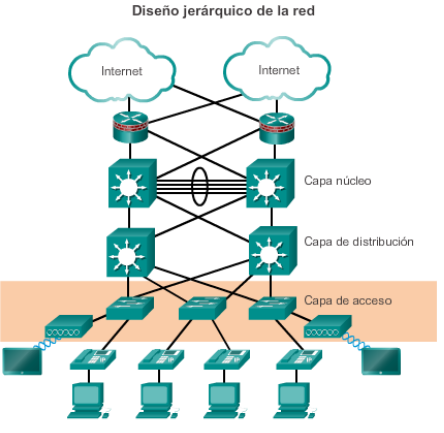
\includegraphics[scale=0.60]{jerarquico}
\end{center}

\subsubsection{ Modelo de n\'ucleo colapsado}
\begin{definicion}[]
{
 combina la capa de distribuci\'on y la capa n\'ucleo
 }
\end{definicion}
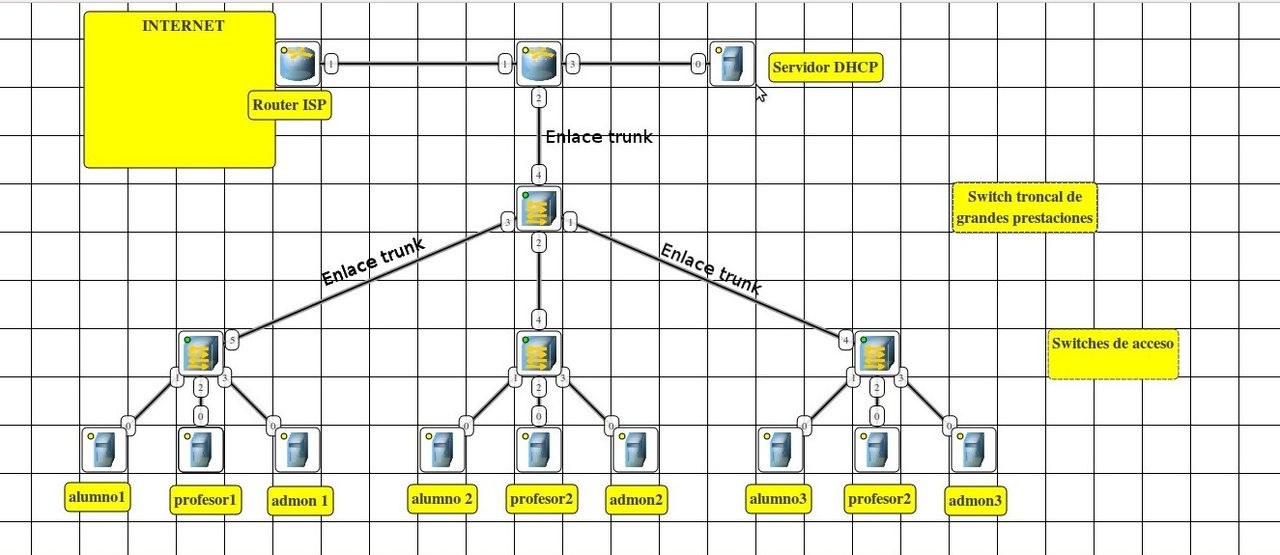
\includegraphics[scale=0.33]{colapsada}

El modelo de dise\~no jer\'arquico es el que implementaremos en el proyecto presente.

\subsection{SEDE AYACUCHO}
\subsubsection{Red central}
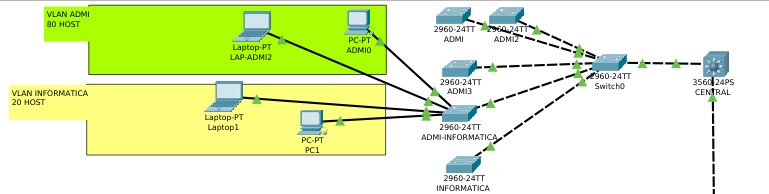
\includegraphics[scale=0.54]{img/central.png} 
\begin{definicion}[]
{
En la red central planteamos dise\~nar un modelo jer\'arquico simple (lo adecuado ser\'ia agregar redundancia en la capa de distribuci\'on). La capa de acceso cuenta con 5 switchs de capa 2(80 host unidad administrativa y 20 unidad inform\'atica). 3 switchs ser\'an propios de vlan admi, 1 ser\'a compartido y 1 ser\'a parcialmente de vlan inform\'atica ya que no alcanza a ocupar todos los puertos disponibles(23 ya que 1 est\'a destinado a conectarse al switch central).El switch central nos permite extender la conectividad ya que con el podemos conectar hasta 23 switches en esta red.
}
\end{definicion}

\subsubsection{Red Campus}
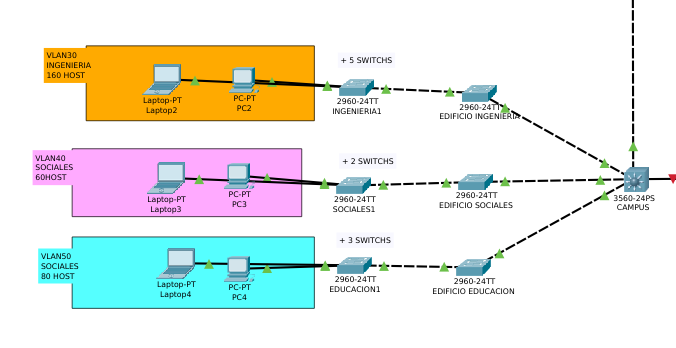
\includegraphics[scale=0.54]{img/CAMPUS.png} 
\begin{definicion}[]
{
En la red del campus se propone hacer una implementaci\'on igual a la anterior, para el primer edificio que cuenta con 160 host se har\'a uso de 160 host que son equivalentes a 7 switchs(23*7), sobrando inclusive 1 puerto.
\\
Para el edificio de sociales se necesitan 60 host para lo cual se hace uso de 3 switchs (3*23), sobrando inclusive 9 puertos.
\\
Para el edificio de educacion que requiere de 80 host se hace uso de 4 switchs (4*23) sobrando inclusive 12 puertos.
}
\end{definicion}




\subsection{SEDE LIMA}
\subsubsection{Red cono sur}
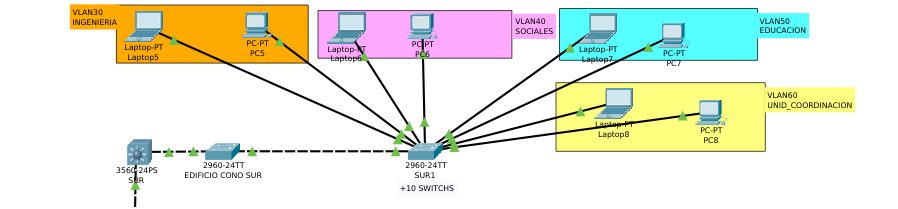
\includegraphics[scale=0.48]{img/CONOSUR.png} 
\begin{definicion}[]
{
Se requiere 240 host por ello, se hace uso de 11 swits (11*23), sobrando 13 puertos.
}
\end{definicion}


\subsubsection{Red cono centro}
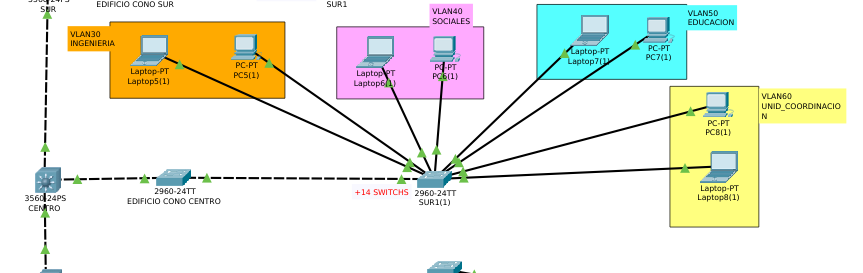
\includegraphics[scale=0.48]{img/CONOCENTRO.png} 
\begin{definicion}[]
{
Se requiere 340 host por ello, se hace uso de 15 swits (15*23), sobrando 5 puertos.
}
\end{definicion}


\subsubsection{Red cono norte}
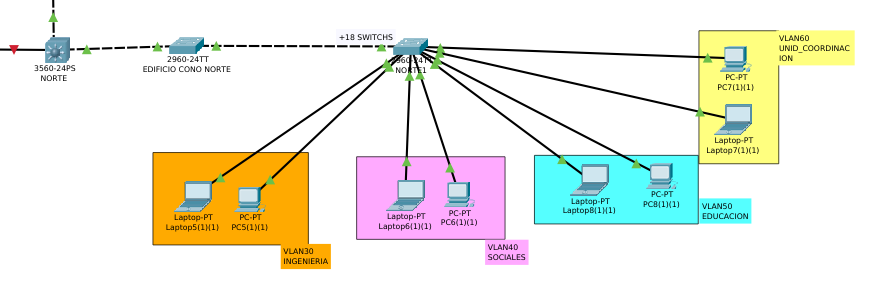
\includegraphics[scale=0.48]{img/CONONORTE.png} 
\begin{definicion}[]
{
Se requiere 420 host por ello, se hace uso de 19 swits (19*23), sobrando 17 puertos.
}
\end{definicion}



\subsection{SEDE HUANCAYO}
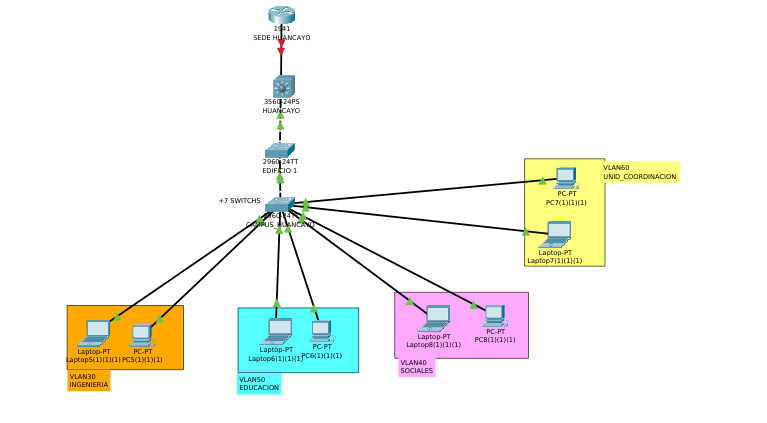
\includegraphics[scale=0.6]{img/HUANCAYO.png} 

\begin{definicion}[]
{
Se requiere 180 host por ello, se hace uso de 8 swits (8*23), sobrando 4 puertos.
}
\end{definicion}

\subsection{SEDE AREQUIPA}
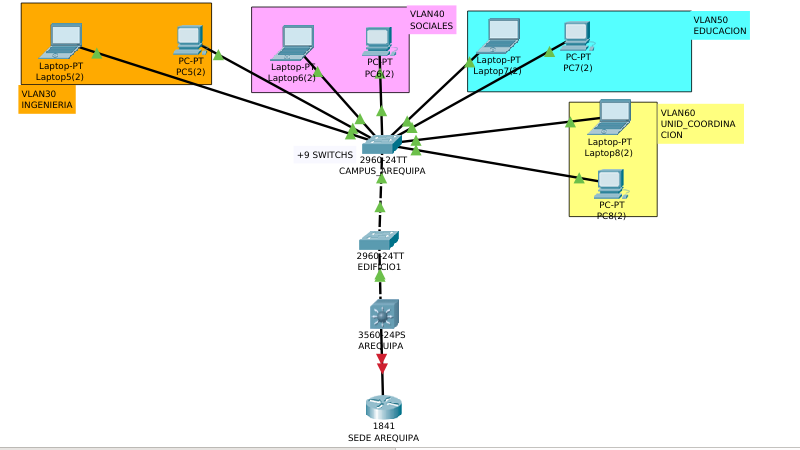
\includegraphics[scale=0.6]{img/AREQUIPA.png} 

\begin{definicion}[]
{
Se requiere 220 host por ello, se hace uso de 10 swits (10*23), sobrando 10 puertos.
}
\end{definicion}


\section{Tipo de direcci\'on IP p\'ublica}
\begin{caja}[]
{
La direcci\'on IP puede ser p\'ublica o privada: La direcci\'on IP p\'ublica es un n\'umero \'unico que identifica nuestra red desde el exterior. La direcci\'on IP privada  identifica a un dispositivo conectado en nuestra red interna.
}
\end{caja}
 Haremos uso de dos tipos de direcciones:
\begin{definicion}[]
{
Direcci\'on externa:
	Direcci\'on externa para la comunicaci\'on de sedes esta direcci\'on es conocida y servir\'a como seguridad para la salida de cada sede. Cada router permitir\'a convertir la direcci\'on interna a la externa al comunicarse a otra sede.
 \\
 Nuestra direcci\'on externa ser\'a 209.165.200.0 que es de tipo c y es la que contratamos.
 }
\end{definicion}
\begin{definicion}[]
{
Direcci\'on Interna:
	Esta direcci\'on es la que segmentaremos para cada sede y esta ser\'a una direcci\'on interna.
 \\
 Nuestra direcci\'on externa ser\'a 172.16.0.0 que es de tipo B.
 }
\end{definicion}


\section{estructura de conexi\'on para la interconexi\'on entre routers}
Se har\'a una conexi\'on NAT con sobrecarga para poder brindar seguridad a la comunicaci\'on entre sedes.\\
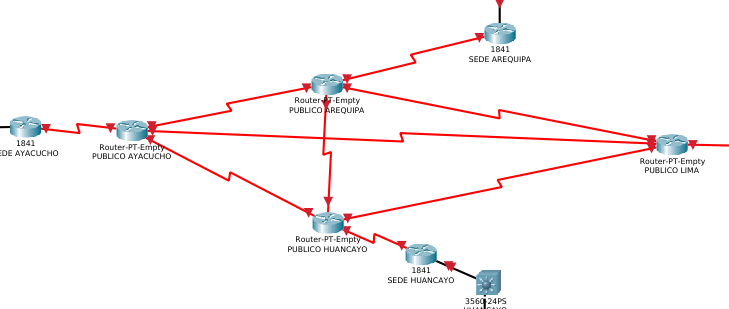
\includegraphics[scale=0.55]{img/ROUTERNAT.png} 

\section{segmentaci\'on de subredes IP}

\subsection{Sede Central Ayacucho}
Usaremos la ip INTERNA: 172.16.0.0
\\
Para hallar usaremos el m\'etodo de VLSM, con el tercer y cuarto octeto. \\

\\
Entonces tenemos:

IP: 172.16.0.0
\\
\textbf{ORDENAMOS LOS HOST QUE SE REQUIERE DE CADA SUCURSAL:}
\\

\begin{definicion}[]
{
\begin{enumerate}[label=\itembolasazules{}]
\item Sede cono-norte: 420 computadoras
\item Sede cono-centro: 340 computadoras
\item Sede campus-ayacucho: 300 computadoras
\item Sede cono-sur: 240 computadoras
\item Sede Arequipa: 220 computadoras
\item Sede Huancayo: 180 computadoras
\item Sede central-ayacucho: 100 computadoras\\
\end{enumerate}
}
\end{definicion}

\newpage
%\usepackage{pdflscape}%poner en vertical hoja en el index
\begin{landscape}
\textheight = 15cm
\textwidth = 25cm % Ancho
\topmargin = -2cm
\oddsidemargin = -1cm
Para poder hacer la segmentaci\'on necesitamos: \\
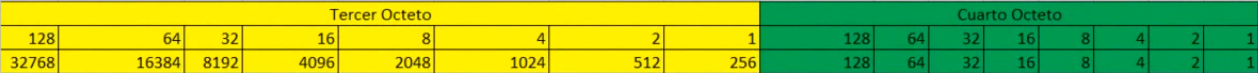
\includegraphics[scale=0.5]{img/octetos.png}
\\
sabemos que la primera subred es la que nos dan por defecto entonces: \\



% Please add the following required packages to your document preamble:
% \usepackage[table,xcdraw]{xcolor}
% If you use beamer only pass "xcolor=table" option, i.e. \documentclass[xcolor=table]{beamer}
\begin{table}[htbp]
\begin{tabular}{|l|l|l|l|l|l|l|}
\hline
\rowcolor[HTML]{32CB00} 
\textbf{subred}  & Host & \textbf{dir sub red} & \textbf{rango ip} & \textbf{broadcast} & \textbf{mascara} & \textbf{/MSR} \\ \hline
cono-norte       & 420  & 172.16.0.0           &                   &                    &                  &               \\ \hline
cono-centro      & 340  &                      &                   &                    &                  &               \\ \hline
campus-ayacucho  & 300  &                      &                   &                    &                  &               \\ \hline
cono-sur         & 240  &                      &                   &                    &                  &               \\ \hline
Arequipa         & 220  &                      &                   &                    &                  &               \\ \hline
Huancayo         & 180  &                      &                   &                    &                  &               \\ \hline
central-Ayacucho & 100  &                      &                   &                    &                  &               \\ \hline
\end{tabular}
\end{table}


Para hallar la siguiente sub red: vemos que requiere 420 host buscamos este numero en la tabla o un valor mayor.
\\
En este caso para 420 es 512; por lo tanto n= 2\\
Quiere decir que la siguiente sub red tendr\'a un salto de 2, asi tenemos:



% Please add the following required packages to your document preamble:
% \usepackage[table,xcdraw]{xcolor}
% If you use beamer only pass "xcolor=table" option, i.e. \documentclass[xcolor=table]{beamer}
\begin{table}[htbp]
\begin{tabular}{|l|l|l|l|l|l|l|}
\hline
\rowcolor[HTML]{32CB00} 
\textbf{subred}  & Host & \textbf{dir sub red} & \textbf{rango ip} & \textbf{broadcast} & \textbf{mascara} & \textbf{/MSR} \\ \hline
cono-norte       & 420  & 172.16.0.0           &                   &                    &                  &               \\ \hline
cono-centro      & 340  & 172.16.2.0           &                   &                    &                  &               \\ \hline
campus-ayacucho  & 300  &                      &                   &                    &                  &               \\ \hline
cono-sur         & 240  &                      &                   &                    &                  &               \\ \hline
Arequipa         & 220  &                      &                   &                    &                  &               \\ \hline
Huancayo         & 180  &                      &                   &                    &                  &               \\ \hline
central-Ayacucho & 100  &                      &                   &                    &                  &               \\ \hline
\end{tabular}
\end{table}


realizamos el mismo paso para los dem\'as:\\
y nos quedaria:


% Please add the following required packages to your document preamble:
% \usepackage[table,xcdraw]{xcolor}
% If you use beamer only pass "xcolor=table" option, i.e. \documentclass[xcolor=table]{beamer}
\begin{table}[htbp]
\begin{tabular}{|l|l|l|l|l|l|l|}
\hline
\rowcolor[HTML]{32CB00} 
\textbf{subred}  & Host & \textbf{dir sub red} & \textbf{rango ip} & \textbf{broadcast} & \textbf{mascara} & \textbf{/MSR} \\ \hline
cono-norte       & 420  & 172.16.0.0           &                   &                    &                  &               \\ \hline
cono-centro      & 340  & 172.16.2.0           &                   &                    &                  &               \\ \hline
campus-ayacucho  & 300  & 172.16.4.0           &                   &                    &                  &               \\ \hline
cono-sur         & 240  & 172.16.6.0           &                   &                    &                  &               \\ \hline
Arequipa         & 220  & 172.16.7.0           &                   &                    &                  &               \\ \hline
Huancayo         & 180  & 172.16.8.0           &                   &                    &                  &               \\ \hline
central-Ayacucho & 100  & 172.16.9.0           &                   &                    &                  &               \\ \hline
\end{tabular}
\end{table}



Para hallar la mascara de sub red lo que hacemos es sumar todos los n\'umeros que esten a la derecha de n incluido n; es decir para la sub red 135.40.0.0 n=2
entonces sumamos: \\
128+64+32+16+8+4+2 = 254\\
Entonces la MSR seria = 255.255.254.0\\
repetimos para todas las sub redes:
% Please add the following required packages to your document preamble:
% \usepackage[table,xcdraw]{xcolor}
% If you use beamer only pass "xcolor=table" option, i.e. \documentclass[xcolor=table]{beamer}
\begin{table}[htbp]
\begin{tabular}{|l|l|l|l|l|l|l|}
\hline
\rowcolor[HTML]{32CB00} 
\textbf{subred}  & Host & \textbf{dir sub red} & \textbf{rango ip} & \textbf{broadcast} & \textbf{mascara} & \textbf{/MSR} \\ \hline
cono-norte       & 420  & 172.16.0.0           &                   &                    & 255.255.254.0    & /23           \\ \hline
cono-centro      & 340  & 172.16.2.0           &                   &                    & 255.255.254.0    & /23           \\ \hline
campus-ayacucho  & 300  & 172.16.4.0           &                   &                    & 255.255.254.0    & /23           \\ \hline
cono-sur         & 240  & 172.16.6.0           &                   &                    & 255.255.255.0    & /24           \\ \hline
Arequipa         & 220  & 172.16.7.0           &                   &                    & 255.255.255.0    & /24           \\ \hline
Huancayo         & 180  & 172.16.8.0           &                   &                    & 255.255.255.0    & /24           \\ \hline
central-Ayacucho & 100  & 172.16.9.0           &                   &                    &                  &               \\ \hline
\end{tabular}
\end{table}

En el caso de la central de ayacucho vemos que se pasa al 4 octeto en ese caso lo que hacemos es buscar ahi un numero >= a 100 entonces n=128 y los que estan a la derecha en el cuarto octeto no seria nadie; por ello quedaria 128\\
Entonces el MSR seria 255.255.255.128\\

% Please add the following required packages to your document preamble:
% \usepackage[table,xcdraw]{xcolor}
% If you use beamer only pass "xcolor=table" option, i.e. \documentclass[xcolor=table]{beamer}
\begin{table}[htbp]
\begin{tabular}{|l|l|l|l|l|l|l|}
\hline
\rowcolor[HTML]{32CB00} 
\textbf{subred}  & Host & \textbf{dir sub red} & \textbf{rango ip} & \textbf{broadcast} & \textbf{mascara} & \textbf{/MSR} \\ \hline
cono-norte       & 420  & 172.16.0.0           &                   &                    & 255.255.254.0    & /23           \\ \hline
cono-centro      & 340  & 172.16.2.0           &                   &                    & 255.255.254.0    & /23           \\ \hline
campus-ayacucho  & 300  & 172.16.4.0           &                   &                    & 255.255.254.0    & /23           \\ \hline
cono-sur         & 240  & 172.16.6.0           &                   &                    & 255.255.255.0    & /24           \\ \hline
Arequipa         & 220  & 172.16.7.0           &                   &                    & 255.255.255.0    & /24           \\ \hline
Huancayo         & 180  & 172.16.8.0           &                   &                    & 255.255.255.0    & /24           \\ \hline
central-Ayacucho & 100  & 172.16.9.0           &                   &                    & 255.255.255.128  & /25           \\ \hline
\end{tabular}
\end{table}


Terminamos de llenar las ips y nos quedaria:

% Please add the following required packages to your document preamble:
% \usepackage[table,xcdraw]{xcolor}
% If you use beamer only pass "xcolor=table" option, i.e. \documentclass[xcolor=table]{beamer}
\begin{table}[htbp]
\begin{tabular}{|l|l|l|l|l|l|l|l|l|}
\hline
\rowcolor[HTML]{32CB00} 
\textbf{subred}  & \textbf{Host} & \textbf{dir sub red} & \textbf{gateway} & \textbf{primer ip} & \textbf{ultimo ip} & \textbf{broadcast} & \textbf{mascara} & \textbf{/MSR} \\ \hline
cono-norte       & 420           & 172.16.0.0           & 172.16.0.1       & 172.16.0.2         & 172.16.1.254       & 172.16.1.255       & 255.255.254.0    & /23           \\ \hline
cono-centro      & 340           & 172.16.2.0           & 172.16.2.1       & 172.16.2.2         & 172.16.3.254       & 172.16.3.255       & 255.255.254.0    & /23           \\ \hline
campus-ayacucho  & 300           & 172.16.4.0           & 172.16.4.1       & 172.16.4.2         & 172.16.5.254       & 172.16.5.255       & 255.255.254.0    & /23           \\ \hline
cono-sur         & 240           & 172.16.6.0           & 172.16.6.1       & 172.16.6.2         & 172.16.6.254       & 172.16.6.255       & 255.255.255.0    & /24           \\ \hline
Arequipa         & 220           & 172.16.7.0           & 172.16.7.1       & 172.16.7.2         & 172.16.7.254       & 172.16.7.255       & 255.255.255.0    & /24           \\ \hline
Huancayo         & 180           & 172.16.8.0           & 172.16.8.1       & 172.16.8.2         & 172.16.8.254       & 172.16.8.255       & 255.255.255.0    & /24           \\ \hline
central-Ayacucho & 100           & 172.16.9.0           & 172.16.9.1       & 172.16.9.2         & 172.16.9.126       & 172.16.9.127       & 255.255.255.128  & /25           \\ \hline
\end{tabular}
\end{table}

\newpage
Para el caso de los Vlans las ip no son lo sufientemente grandes para poder realizar el routing inter vlans y no nos deja crear las subinterfaces de vlans. Por ello se volvi\'o a realizar el c\'alculo considerando las VLAN\' s haciendo uso de una herramienta web: \\ 
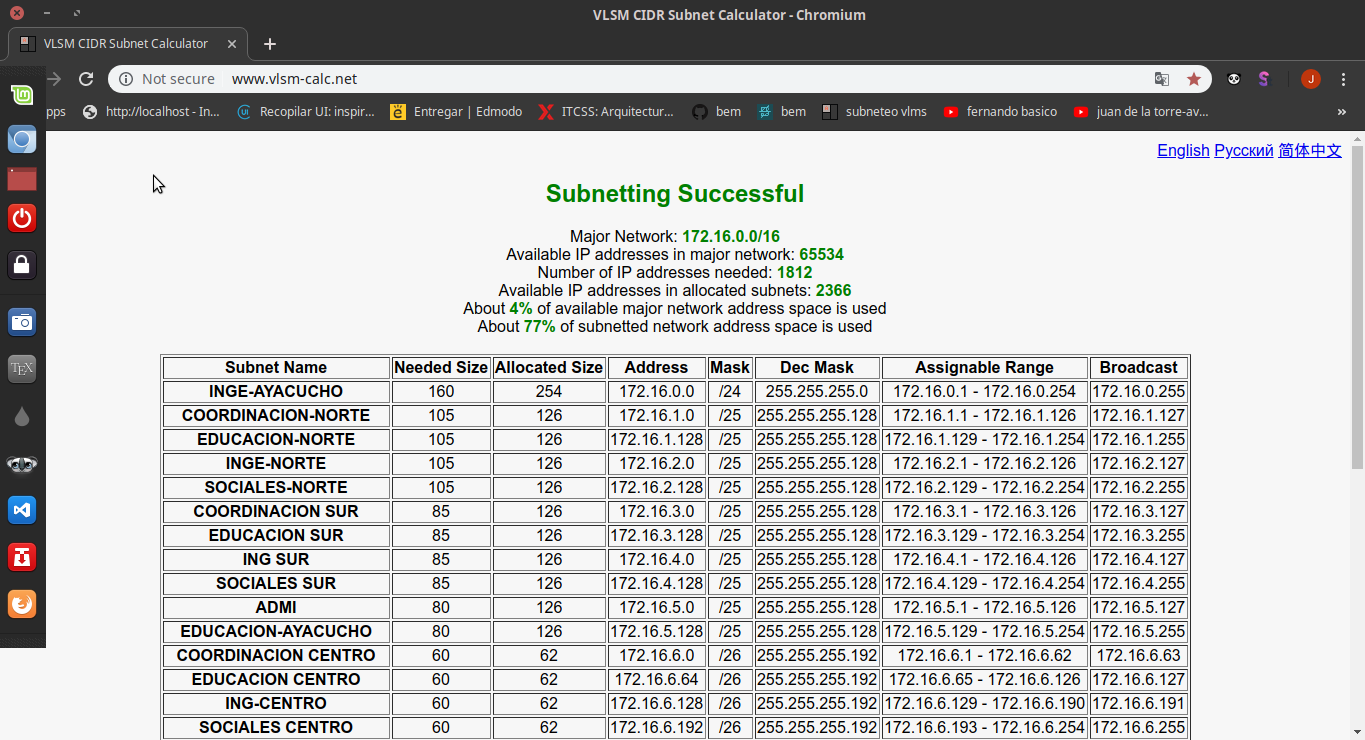
\includegraphics[scale=0.44]{img/vlsm-calc.png}\\
Quedando la tabla como se muestra a continuaci\'on:


\end{landscape}
\\

% Please add the following required packages to your document preamble:
% \usepackage[table,xcdraw]{xcolor}
% If you use beamer only pass "xcolor=table" option, i.e. \documentclass[xcolor=table]{beamer}
\begin{table}[htbp]
\begin{tabular}{|l|l|l|l|l|l|}
\hline
\rowcolor[HTML]{34FF34} 
\textbf{subred}      & \textbf{hosts} & \textbf{Direccion} & \textbf{/MSR} & \textbf{MASCARA} & \textbf{Rango}              \\ \hline
ing ayacucho         & 160            & 172.16.0.0         & / 24          & 255.255.255.0    & 172.16.0.1 - 172.16.0.254   \\ \hline
coor norte           & 105            & 172.16.1.0         & / 25          & 255.255.255.128  & 172.16.1.1 - 172.16.1.126   \\ \hline
edu norte      & 105            & 172.16.1.128       & / 25          & 255.255.255.128  & 172.16.1.129 - 172.16.1.254 \\ \hline
inge norte           & 105            & 172.16.2.0         & / 25          & 255.255.255.128  & 172.16.2.1 - 172.16.2.126   \\ \hline
soc norte         & 105            & 172.16.2.128       & / 25          & 255.255.255.128  & 172.16.2.129 - 172.16.2.254 \\ \hline
coord sur            & 85             & 172.16.3.0         & / 25          & 255.255.255.128  & 172.16.3.1 - 172.16.3.126   \\ \hline
edu sur        & 85             & 172.16.3.128       & / 25          & 255.255.255.128  & 172.16.3.129 - 172.16.3.254 \\ \hline
ing sur              & 85             & 172.16.4.0         & / 25          & 255.255.255.128  & 172.16.4.1 - 172.16.4.126   \\ \hline
soc sur         & 85             & 172.16.4.128       & / 25          & 255.255.255.128  & 172.16.4.129 - 172.16.4.254 \\ \hline
admi                 & 80             & 172.16.5.0         & / 25          & 255.255.255.128  & 172.16.5.1 - 172.16.5.126   \\ \hline
edu ayacucho   & 80             & 172.16.5.128       & / 25          & 255.255.255.128  & 172.16.5.129 - 172.16.5.254 \\ \hline
Coor centro & 60             & 172.16.6.0         & / 26          & 255.255.255.192  & 172.16.6.1 - 172.16.6.62    \\ \hline
edu centro    & 60             & 172.16.6.64        & / 26          & 255.255.255.192  & 172.16.6.65 - 172.16.6.126  \\ \hline
inge centro          & 60             & 172.16.6.128       & / 26          & 255.255.255.192  & 172.16.6.129 - 172.16.6.190 \\ \hline
soc centro      & 60             & 172.16.6.192       & / 26          & 255.255.255.192  & 172.16.6.193 - 172.16.6.254 \\ \hline
soc ayacucho    & 60             & 172.16.7.0         & / 26          & 255.255.255.192  & 172.16.7.1 - 172.16.7.62    \\ \hline
coord arequipa       & 55             & 172.16.7.64        & / 26          & 255.255.255.192  & 172.16.7.65 - 172.16.7.126  \\ \hline
edu arequipa       & 55             & 172.16.7.128       & / 26          & 255.255.255.192  & 172.16.7.129 - 172.16.7.190 \\ \hline
ing arequipa         & 55             & 172.16.7.192       & / 26          & 255.255.255.192  & 172.16.7.193 - 172.16.7.254 \\ \hline
soc arequipa    & 55             & 172.16.8.0         & / 26          & 255.255.255.192  & 172.16.8.1 - 172.16.8.62    \\ \hline
coord huancayo       & 45             & 172.16.8.64        & / 26          & 255.255.255.192  & 172.16.8.65 - 172.16.8.126  \\ \hline
edu huancayo     & 45             & 172.16.8.128       & / 26          & 255.255.255.192  & 172.16.8.129 - 172.16.8.190 \\ \hline
inge huancayo        & 45             & 172.16.8.192       & / 26          & 255.255.255.192  & 172.16.8.193 - 172.16.8.254 \\ \hline
soc huancayo    & 45             & 172.16.9.0         & / 26          & 255.255.255.192  & 172.16.9.1 - 172.16.9.62    \\ \hline
informatica          & 20             & 172.16.9.64        & / 27          & 255.255.255.224  & 172.16.9.65 - 172.16.9.94   \\ \hline
servidor central     & 3              & 172.16.9.96        & / 29          & 255.255.255.248  & 172.16.9.97 - 172.16.9.102  \\ \hline
router arequipa      & 2              & 172.16.9.104       & / 30          & 255.255.255.252  & 172.16.9.105 - 172.16.9.106 \\ \hline
router ayacucho      & 2              & 172.16.9.108       & / 30          & 255.255.255.252  & 172.16.9.109 - 172.16.9.110 \\ \hline
router huancayo      & 2              & 172.16.9.112       & / 30          & 255.255.255.252  & 172.16.9.113 - 172.16.9.114 \\ \hline
router lima          & 2              & 172.16.9.116       & / 30          & 255.255.255.252  & 172.16.9.117 - 172.16.9.118 \\ \hline
servidor lima        & 1              & 172.16.9.120       & / 30          & 255.255.255.252  & 172.16.9.121 - 172.16.9.122 \\ \hline
\end{tabular}
\end{table}

\section{segmentaci\'on de subredes VLAN}

Realizaremos la segmentaci\'on por puertos, con las nuevas subredes que hallamos\\
\subsection{Ayacucho}

\subsubsection{sede central administrativa}
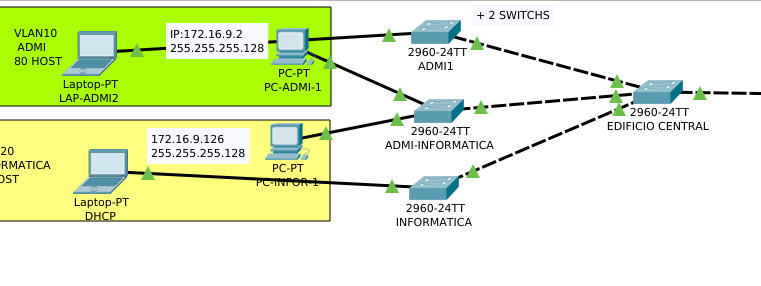
\includegraphics[scale=0.42]{img/vlancentral.png} 

\\comprobamos que funciona\\
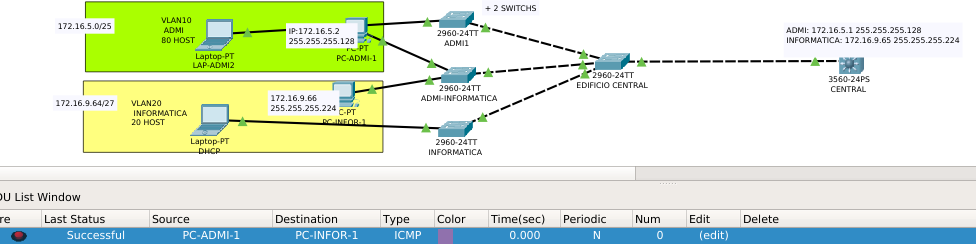
\includegraphics[scale=0.45]{img/vlan100sucess.png} 
 
 \subsubsection{Campus Universitario}
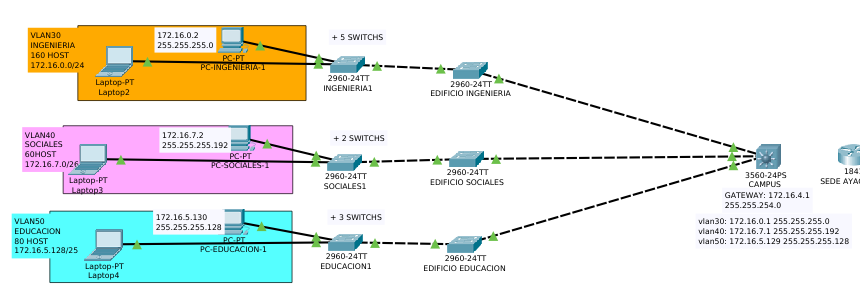
\includegraphics[scale=0.45]{img/VLANCAMPUS.png} 
\\comprobamos que funciona\\

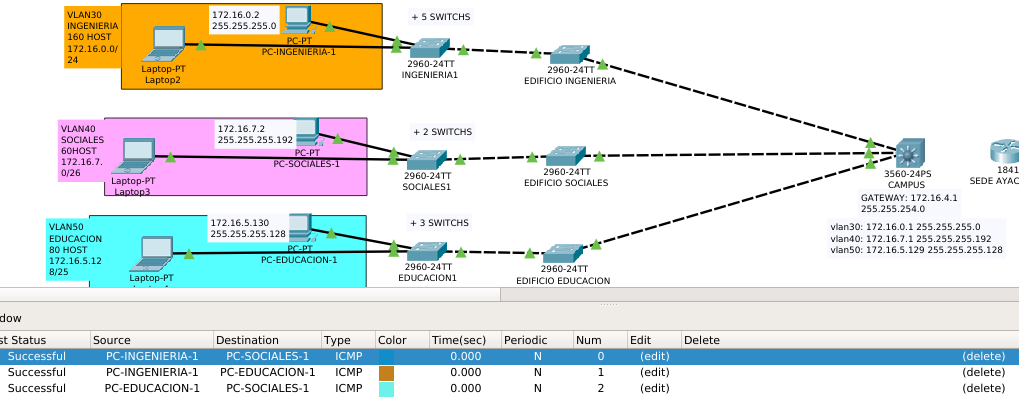
\includegraphics[scale=0.5]{img/VLANCAMPUSSUCESS.png} 
\subsection{Conexi\'on sucursal Lima}
\subsubsection{sucursal cono norte}
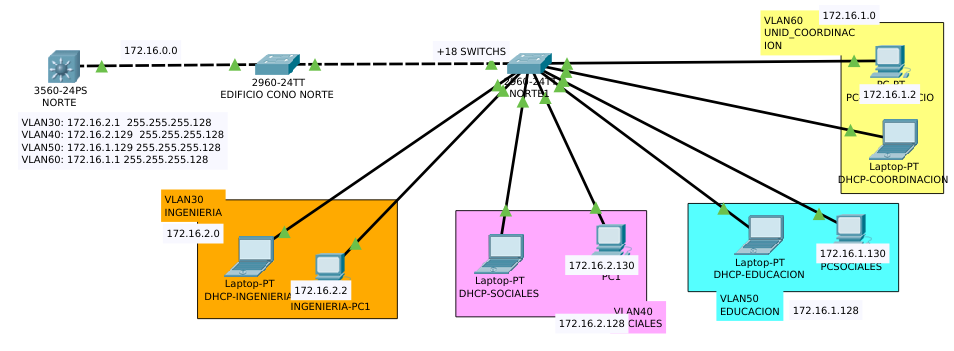
\includegraphics[scale=0.45]{img/VLANNORTE.png} \\
\\comprobamos que funciona\\
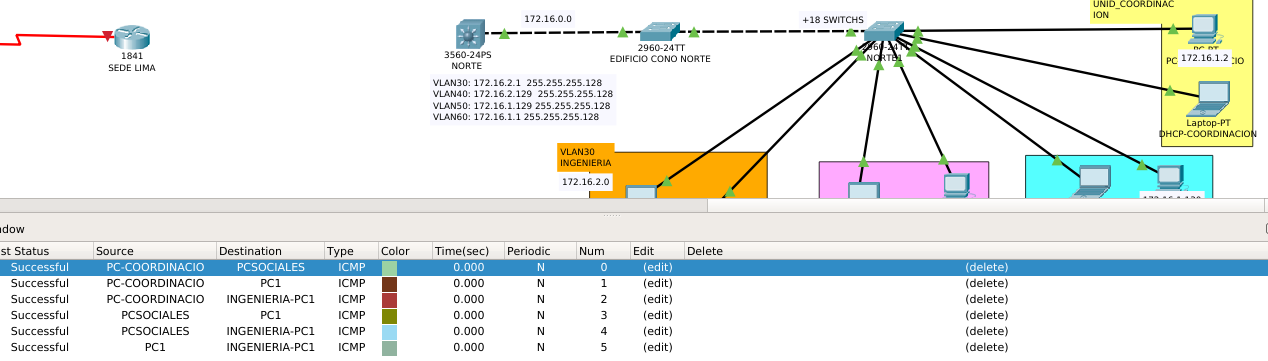
\includegraphics[scale=0.35]{img/NORTESUCCESS.png} 
\subsubsection{sucursal cono centro}
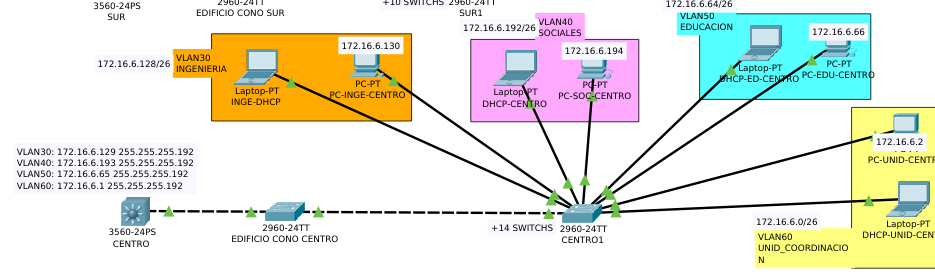
\includegraphics[scale=0.45]{img/VLANCENTRO.png} 
\\comprobamos que funciona\\
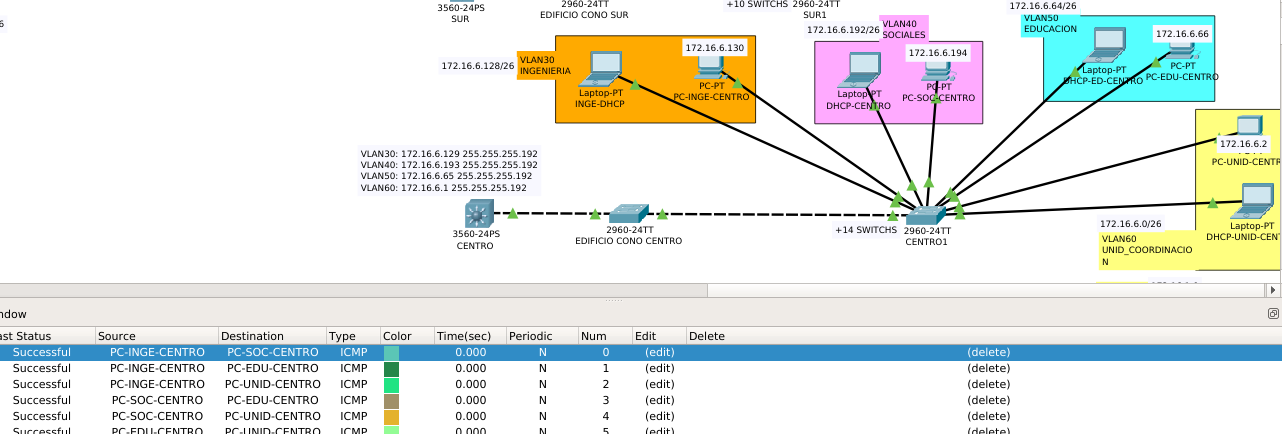
\includegraphics[scale=0.35]{img/centrosucess.png} 
\subsubsection{sucursal cono sur}
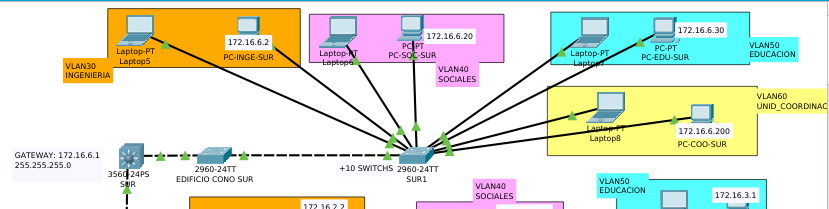
\includegraphics[scale=0.45]{img/VLANSUR.png} 
\\comprobamos que funciona\\
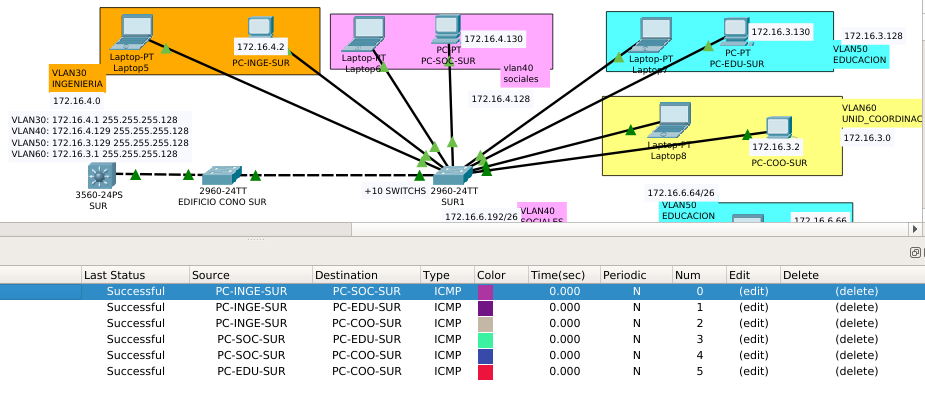
\includegraphics[scale=0.45]{img/sursucess.png} 

\subsection{Conexi\'on sucursal Arequipa}
ser\'an de igual manera que de la sucursal de lima.
\\
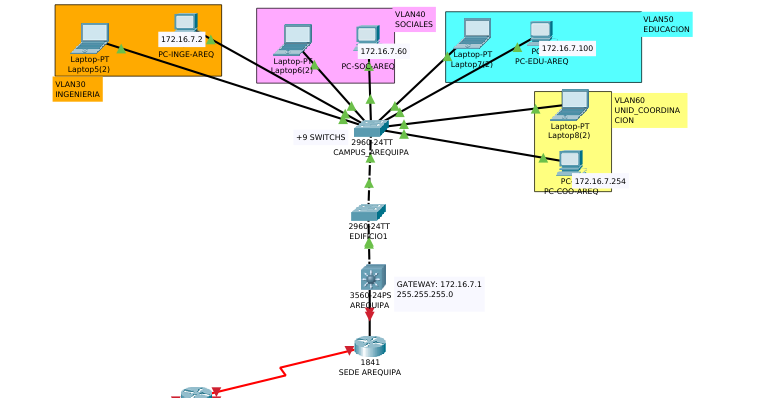
\includegraphics[scale=0.45]{img/VLANAREQUIPA.png} 
\\comprobamos que funciona
\\
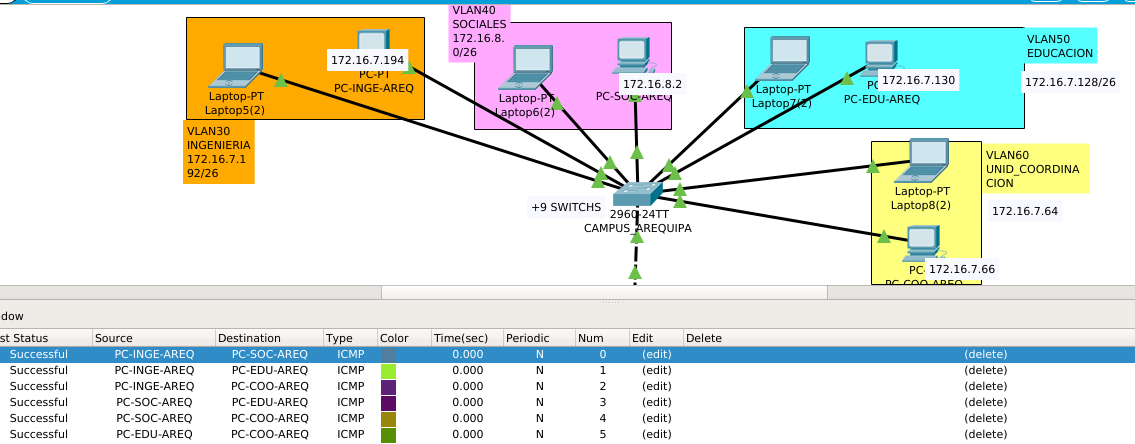
\includegraphics[scale=0.4]{img/arequipasucess.png} 

\subsection{Conexi\'on sucursal Huancayo}
ser\'an de igual manera que de la sucursal de lima.
\\
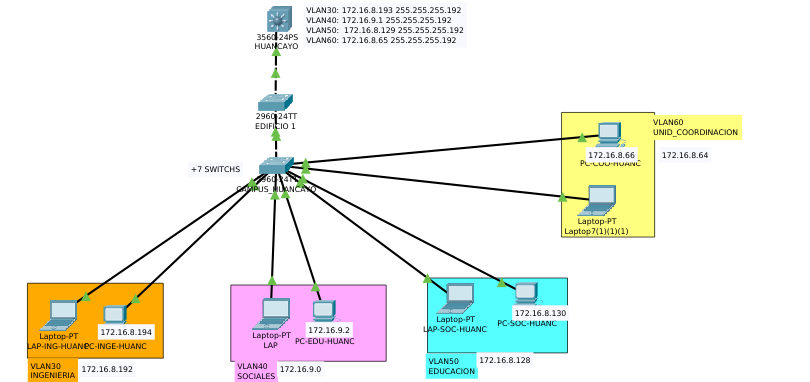
\includegraphics[scale=0.45]{img/VLANHUANCAYO.png} 
\\comprobamos que funciona
\\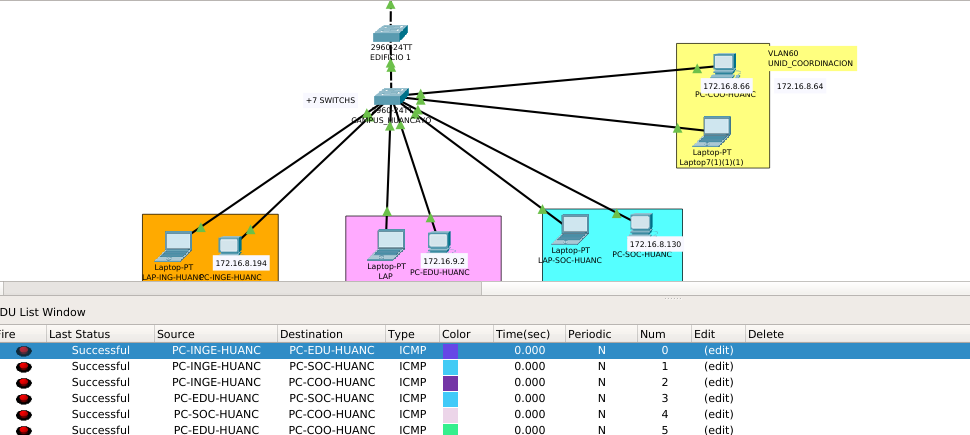
\includegraphics[scale=0.45]{img/HUANCAYOSUCESS.png} 

\section{\¿Le parece acertada la decisi\'on del Jefe de Inform\'atica?, Sustente en profundidad su respuesta para cada caso}
\subsection{SEGMENTACI\'ON DE REDES}
\begin{definicion}[]
{
\begin{enumerate}[label=\itembolasazules{}]
\item Qu\'e se adquiera una direcci\'on IP p\'ublica y que se utilice
segmentaci\'on basada en subredes IP para cada una de las sucursales.
\item Qu\'e cada una de las Facultades sean segmentadas utilizando VLAN.
\end{enumerate}
}
\end{definicion}
Para este caso la utilizaci\'on de una ip publica mejora mucho la seguridad de una red ya que al salir hacia una wan o internet estamos propensos a sufrir suplantacion de identidad entre muchas otras cosas.
\\
la ip publica hace que esto sea mas dificil de realizar ya q siempre saldremos al exterior con una ip publica de conocimiento de todos.\\

NO solo las facultades deben de ser segmentadas en Vlans sino todas las unidades involucradas para poder tener asi un mejor control en la red.
\subsection{LOCALIZACI\'ON DE SERVIDORES}
\begin{definicion}[]
{
\begin{enumerate}[label=\itembolasazules{}]
\item Que la Oficina de Inform\'atica en Ayacucho tenga.

\begin{enumerate}[label=\itembolas{}]
\item 01 Servidor de DHCP, que asigne direcciones IP din\'amicas a las
sedes de Ayacucho, Arequipa y Huancayo.
\item 1 Servidor de DNS.
\item 1 Servidor Web que contenga las p\'aginas web de cada una de las
sedes (Ayacucho, Lima, Arequipa y Huancayo).
\end{enumerate}

\item Qu\'e la Sede Lima Cono Central tenga: 01 Servidor para servicio de DHCP, que asigne direcciones IP
din\'amicas a las tres sedes de Lima solamente.
\end{enumerate}
}

\end{definicion}
Lo mas recomendable deber\'ia ser tener todos esos servidores en un ambiente m\'as adecuado, ya que no se menciona que la casona cuente con lo requerido para que se cumplan los est\'andares basicos que se requiere.
\\
Se deberia de separar con una granja de servidores y asi provea servicio a todos; los servidores deber\'ian de estar ubicados todos juntos en un lugar adecuado.

